% Small-angle scattering and the impulse approximation (attractive case, V = -GMm/r).
% Left: true orbit (green; numerically integrated with k = GM/v^2 = 0.15 b, theta = 17 deg,
%       deflection exaggerated) vs the straight path y = b (gray dashed) used in the
%       impulse approximation. Forces on the straight path at vt = -b, 0, +b (|F| ~ 1/r^2):
%       F_parallel (dashed) cancels between t and -t, F_perp (solid) adds up.
% Right: F_perp(t) ~ (1+v^2t^2/b^2)^{-3/2},  F_parallel(t) ~ -(vt/b)(1+v^2t^2/b^2)^{-3/2}
%       (positive = along v). Shaded area = Delta p_perp; the F_parallel integral vanishes.
% Compile: pdflatex impulse_tikz.tex
\documentclass[tikz,border=6pt]{standalone}
\usepackage{amsmath}
\usepackage{fix-cm}
\usetikzlibrary{arrows.meta}
\begin{document}
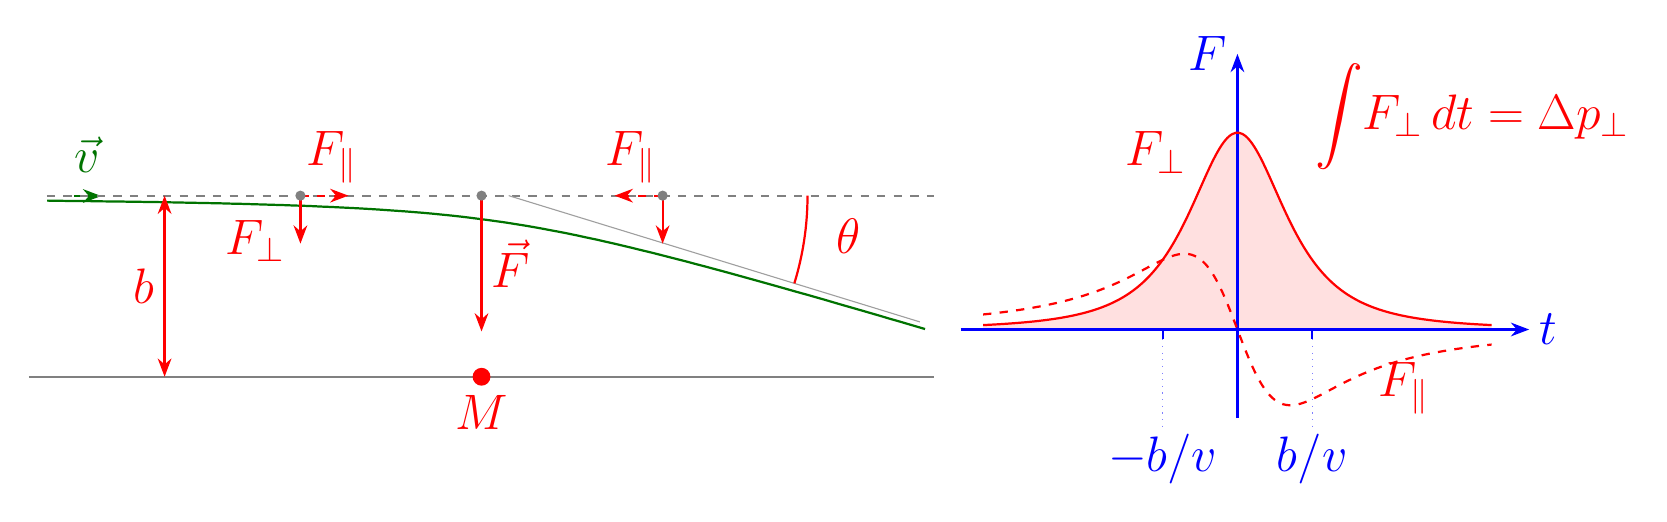
\begin{tikzpicture}[>=Stealth,thick,every node/.style={font=\fontsize{18}{22}\selectfont}]
  % ---------------- left panel: geometry ----------------
  \begin{scope}[scale=1.15]
  \draw[gray] (-5.0,0) -- (5.0,0);
  \fill[red] (0,0) circle (2.8pt);
  \node[red,below=3pt] at (0,0) {$M$};
  % true orbit
  \draw[green!45!black] plot[smooth] coordinates {(-4.798,1.945) (-4.697,1.944) (-4.595,1.942) (-4.494,1.941) (-4.392,1.940) (-4.290,1.939) (-4.188,1.937) (-4.086,1.936) (-3.986,1.935) (-3.886,1.933) (-3.786,1.932) (-3.685,1.930) (-3.585,1.929) (-3.484,1.927) (-3.383,1.925) (-3.282,1.923) (-3.181,1.921) (-3.080,1.919) (-2.978,1.917) (-2.877,1.915) (-2.775,1.912) (-2.673,1.910) (-2.573,1.907) (-2.472,1.904) (-2.372,1.901) (-2.271,1.898) (-2.170,1.895) (-2.069,1.891) (-1.968,1.888) (-1.866,1.884) (-1.764,1.879) (-1.662,1.875) (-1.562,1.870) (-1.462,1.865) (-1.361,1.860) (-1.260,1.854) (-1.159,1.848) (-1.057,1.841) (-0.956,1.834) (-0.854,1.827) (-0.754,1.819) (-0.653,1.811) (-0.553,1.802) (-0.452,1.792) (-0.351,1.782) (-0.250,1.771) (-0.149,1.759) (-0.048,1.746) (0.053,1.733) (0.154,1.719) (0.255,1.705) (0.356,1.689) (0.457,1.673) (0.557,1.656) (0.658,1.638) (0.758,1.619) (0.860,1.600) (0.961,1.580) (1.063,1.559) (1.163,1.537) (1.264,1.516) (1.364,1.493) (1.466,1.470) (1.567,1.446) (1.668,1.422) (1.769,1.397) (1.869,1.373) (1.972,1.347) (2.073,1.321) (2.175,1.295) (2.276,1.269) (2.376,1.242) (2.476,1.216) (2.579,1.188) (2.680,1.161) (2.782,1.133) (2.883,1.105) (2.984,1.077) (3.085,1.049) (3.185,1.021) (3.285,0.993) (3.387,0.964) (3.489,0.935) (3.591,0.907) (3.692,0.878) (3.794,0.849) (3.895,0.819) (3.995,0.790) (4.096,0.761) (4.197,0.732) (4.297,0.703) (4.397,0.674) (4.497,0.644) (4.599,0.615) (4.701,0.585) (4.803,0.555) (4.898,0.527)};
  \draw[green!45!black,->] (-4.5,1.996) -- (-4.2,1.996);
  \node[green!45!black] at (-4.35,2.45) {$\vec v$};
  % straight-line path (impulse approximation) and outgoing asymptote
  \draw[gray,dashed] (-4.8,2) -- (5.0,2);
  \draw[gray!75,thin] (0.30,2) -- ({0.30+4.75*cos(17.07)},{2-4.75*sin(17.07)});
  \draw[red] (3.6,2) arc[start angle=0,end angle=-17.07,radius=3.3];
  \node[red] at (4.05,1.55) {$\theta$};
  % impact parameter
  \draw[red,<->] (-3.5,0) -- (-3.5,2) node[midway,left] {$b$};
  % forces on the straight path: t = 0
  \draw[red,->] (0,2) -- (0,0.5) node[midway,right] {$\vec F$};
  % t = -b/v and t = +b/v : |F| = 1.5/2, components 0.53
  \draw[red,->] (-2,2) -- (-2,1.47);
  \draw[red,dashed,->] (-2,2) -- (-1.47,2);
  \draw[red,->] (2,2) -- (2,1.47);
  \draw[red,dashed,->] (2,2) -- (1.47,2);
  \node[red] at (-2.5,1.5) {$F_\perp$};
  \node[red] at (-1.65,2.42) {$F_\parallel$};
  \node[red] at (1.65,2.42) {$F_\parallel$};
  \fill[gray] (-2,2) circle (1.6pt) (0,2) circle (1.6pt) (2,2) circle (1.6pt);
  \end{scope}

  % ---------------- right panel: F(t) ----------------
  \begin{scope}[xshift=9.6cm,yshift=0.6cm,x=0.95cm,y=2.5cm]
    \fill[red!12] plot[domain=-3.4:3.4,samples=150,smooth] (\x,{1/(1+\x*\x)^1.5}) -- (3.4,0) -- (-3.4,0) -- cycle;
    \draw[blue,->] (-3.7,0) -- (3.9,0) node[right] {$t$};
    \draw[blue,->] (0,-0.45) -- (0,1.4) node[left] {$F$};
    \foreach \x/\l in {-1/{-b/v},1/{b/v}} {
      \draw[blue] (\x,0) -- (\x,-.05);
      \draw[blue!50,thin,dotted] (\x,-.05) -- (\x,-.5);
      \node[blue] at (\x,-.66) {$\l$};}
    \draw[red,domain=-3.4:3.4,samples=150,smooth] plot (\x,{1/(1+\x*\x)^1.5});
    \draw[red,dashed,domain=-3.4:3.4,samples=150,smooth] plot (\x,{-\x/(1+\x*\x)^1.5});
    \node[red,anchor=east] at (-0.55,0.9) {$F_\perp$};
    \node[red,anchor=west] at (1.75,-0.3) {$F_\parallel$};
    \node[red,anchor=west] at (0.9,1.08) {$\displaystyle\int\! F_\perp\,dt=\Delta p_\perp$};
  \end{scope}
\end{tikzpicture}
\end{document}
